\documentclass[aps,pre,onecolumn,10pt,groupedaddress,amsmath,amssymb,floatfix]{revtex4-2}

\usepackage{graphicx}
\graphicspath{{figures/}}
\usepackage{dcolumn}
\usepackage{bm}
\usepackage{hyperref}
\usepackage{amsthm}

\newtheorem{theorem}{Theorem}
\newtheorem{lemma}{Lemma}
\newtheorem{definition}{Definition}
\newtheorem{proposition}{Proposition}
\newtheorem{corollary}{Corollary}
\newtheorem{remark}{Remark}

\begin{document}

\title{An Exact Rational Invariant for Forman--Ricci Curvature on Chebyshev Toroidal Lattices}

\author{Juan Carlos Alves Tabernero}
\email{cienciasolar@gmx.com}
\affiliation{Independent Researcher, Salamanca, Spain}

\date{\today}

\begin{abstract}
Discrete curvature notions provide a natural bridge between combinatorial topology and Riemannian geometry. We study the Forman--Ricci curvature on three-dimensional toroidal lattices governed by the Chebyshev ($\ell^\infty$) metric, as a function of the integer interaction range $\lambda \ge 1$. We derive a closed-form analytical expression for the mean curvature per edge, valid for any torus size $L \ge 4\lambda$ in the no-aliasing regime. The formula reads
$\langle\kappa_e\rangle(\lambda) = -\frac{47\lambda^5 + 141\lambda^4 + 156\lambda^3 + 85\lambda^2 + 24\lambda + 3}{2(4\lambda^2 + 6\lambda + 3)}$.
From this expression we construct a dimensionless invariant
$\mathcal{I}(\lambda) = |\langle\kappa_e\rangle| \lambda^3 / k(\lambda)^2$,
where $k(\lambda) = (2\lambda+1)^3 - 1$ is the vertex degree. We prove that this invariant is the unique adimensional bilinear coupling of curvature, coordination volume, and squared connectivity that remains finite and rational in the dense limit. In the asymptotic regime $\lambda \to \infty$, the invariant converges to the exact rational number
$\mathcal{I}_\infty = 47/512 \approx 0.091796875$.
We further show that $47/512$ is an intrinsic geometric constant of the continuum $\ell^\infty$ metric on the three-torus, equal to the ratio of the asymptotic curvature coefficient $C_\kappa = -47/8$ to the squared asymptotic degree coefficient $C_k^2 = 64$, both obtained by exact integration of overlapping $\ell^\infty$ unit balls. All analytical results are independently validated by symbolic, brute-force, and high-precision numerical computations. The paper makes no claim of connection to quantum gravity or of convergence to smooth Riemannian geometry.
\end{abstract}

\maketitle

% ============================================================================
% 1. INTRODUCTION
% ============================================================================
\section{Introduction}
\label{sec:intro}

The study of discrete curvature on graphs and lattices has become a central topic in discrete differential geometry \cite{chung1997spectral, chapman2013curvature, jost2014ollivier, bridson1999metric}, with applications ranging from network science \cite{weber2017forman, samal2018comparative, albert2002statistical} to lattice gauge theory \cite{kogut1979introduction, wilson1974confinement, goldenfeld1992lectures}. Two combinatorial notions of curvature have become standard: Ollivier--Ricci curvature \cite{ollivier2009ricci}, based on optimal transport between neighbourhoods, and Forman--Ricci curvature \cite{forman2003bochner}, based on combinatorial cell complexes. Forman--Ricci curvature has the practical advantage of being a purely combinatorial, transport-free quantity, evaluated locally on each edge as a linear combination of vertex degrees and the number of triangles sharing the edge. It has been applied extensively to complex networks \cite{sreejith2016forman}, community detection \cite{sandhu2016ricci}, and biological systems \cite{gosztolai2021unfolding}, and it is closely related to spectral graph theory \cite{chung1997spectral}.

Historically, discrete models of geometry have also been studied in the context of quantum gravity, where frameworks such as loop quantum gravity \cite{ashtekar2004background}, causal dynamical triangulations \cite{ambjorn2012nonperturbative}, and causal set theory \cite{surya2019causal} replace the smooth Lorentzian manifold by a combinatorial structure. The connection between discrete curvature and smooth Riemannian geometry is well established \cite{misner1973gravitation, hamilton1982three, docarmo1992riemannian}. The present work is not a contribution to those programs; we mention them only as historical context. Our focus is the mathematical study of Forman--Ricci curvature on a specific class of lattices.

Despite the extensive application of Forman--Ricci curvature to complex networks, exact closed-form results on regular spatial lattices with extended interaction ranges remain scarce. Most studies rely on numerical diagonalisation or nearest-neighbour approximations, leaving the dense asymptotic regime $\lambda \to \infty$ largely unexplored analytically. The Chebyshev ($\ell^\infty$) lattice is particularly suited to analytical treatment because its coordination geometry is a solid cube, whose intersection volume factorises over the three coordinate axes, allowing exact computations that would be intractable for other metrics \cite{conway1999sphere, thompson1996minkowski}. This makes the Chebyshev lattice the natural setting in which an exact closed-form curvature invariant can be derived.

In this paper we perform a rigorous study of Forman--Ricci curvature on three-dimensional toroidal Chebyshev networks. Our main contributions are fourfold:
\begin{enumerate}
\item We define the graph-theoretical structure of the 3D toroidal Chebyshev lattice with integer interaction range $\lambda$, and establish its metric and symmetry properties.
\item We derive an exact closed-form expression for the mean Forman--Ricci curvature $\langle\kappa_e\rangle(\lambda)$, valid for all $\lambda \ge 1$ in the no-aliasing regime $L \ge 4\lambda$.
\item We construct a dimensionless invariant $\mathcal{I}(\lambda)$ and prove its uniqueness under a dual-normalisation scaling argument.
\item We show that in the dense limit $\lambda \to \infty$, the invariant converges to the exact rational number $\mathcal{I}_\infty = 47/512$, and we identify its geometric origin as an intrinsic integral constant of the $\ell^\infty$ metric on $\mathbb{T}^3$.
\end{enumerate}

The paper is organised as follows. Section~\ref{sec:network} defines the Chebyshev network and its metric properties. Section~\ref{sec:forman} reviews Forman--Ricci curvature and its structure on regular lattices. Section~\ref{sec:closed_form} derives the closed-form expression for $\langle\kappa_e\rangle(\lambda)$. Section~\ref{sec:invariant} proves the uniqueness of the invariant and establishes the geometric limit $47/512$. Section~\ref{sec:discussion} discusses implications, scope, and open problems. Section~\ref{sec:conclusions} summarises.

% ============================================================================
% 2. THE CHEBYSHEV NETWORK
% ============================================================================
\section{The Chebyshev network}
\label{sec:network}

\subsection{Graph construction}

Let $\mathbb{T}^3_L = (\mathbb{Z}/L\mathbb{Z})^3$ denote the three-dimensional discrete torus of side length $L \in \mathbb{N}^+$, with $N = L^3$ nodes. Each node $\mathbf{u} \in \mathbb{T}^3_L$ is identified by integer coordinates $\mathbf{u} = (u_1, u_2, u_3)$ modulo $L$.

\begin{definition}[Toroidal Chebyshev distance]
The Chebyshev ($\ell^\infty$) distance on the torus between two nodes $\mathbf{u}, \mathbf{v} \in \mathbb{T}^3_L$ is
\begin{equation}
d_\infty(\mathbf{u}, \mathbf{v}) = \max_{i \in \{1,2,3\}} \min\left(|u_i - v_i|, L - |u_i - v_i|\right).
\label{eq:cheb_dist}
\end{equation}
\end{definition}

\begin{lemma}[Metric property]
$d_\infty$ is a metric on $\mathbb{T}^3_L$.
\end{lemma}
\begin{proof}
Non-negativity and symmetry are immediate. The identity of indiscernibles follows from $d_\infty(\mathbf{u}, \mathbf{v}) = 0 \iff u_i = v_i$ for all $i$. For the triangle inequality, write $d_\infty(\mathbf{u}, \mathbf{v}) = \min_{\mathbf{n} \in \mathbb{Z}^3} \|\mathbf{u} - \mathbf{v} + L\mathbf{n}\|_\infty$, where $\|\cdot\|_\infty$ is the usual $\ell^\infty$ norm on $\mathbb{R}^3$ \cite{rudin1991functional}. Then for any $\mathbf{u}, \mathbf{v}, \mathbf{w}$ and optimal lattice shifts $\mathbf{m}, \mathbf{n}$,
\[
\|\mathbf{u} - \mathbf{v} + L\mathbf{m}\|_\infty + \|\mathbf{v} - \mathbf{w} + L\mathbf{n}\|_\infty \geq \|\mathbf{u} - \mathbf{w} + L(\mathbf{m}+\mathbf{n})\|_\infty,
\]
which by the usual triangle inequality in $\mathbb{R}^3$ gives the result.
\end{proof}

\begin{definition}[Chebyshev lattice graph]
For a fixed integer interaction range $\lambda \ge 1$, the Chebyshev graph $G(L, \lambda) = (V, E)$ has vertex set $V = \mathbb{T}^3_L$ and edge set
\begin{equation}
E = \{\{u, v\} \subseteq V \mid 0 < d_\infty(\mathbf{u}, \mathbf{v}) \le \lambda\}.
\label{eq:edges}
\end{equation}
\end{definition}

For $\lambda = 1$, the resulting graph is $26$-valent on the 3D torus, with each node connected to its 26 nearest neighbours in the $\ell^\infty$ sense. The coordination cube and the three neighbour types are illustrated in Fig.~\ref{fig:network}. The graph-theoretic structure of $G(L, \lambda)$ is analysed in detail in the classic monograph by Bollobás \cite{bollobas1998modern}.

\begin{figure}[htbp]
\centering
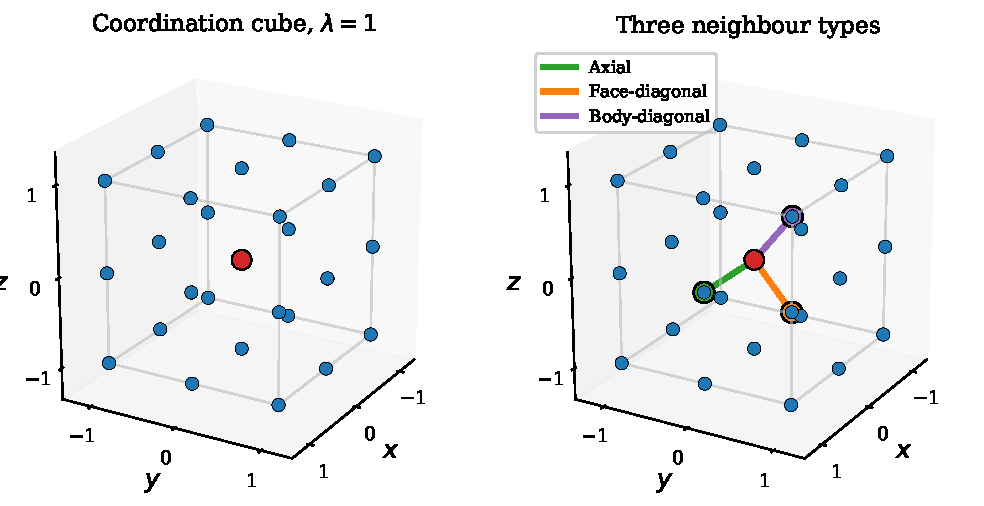
\includegraphics[width=0.8\linewidth]{figure1_network.pdf}
\caption{
Schematic of the Chebyshev coordination cube for interaction range
$\lambda = 1$. Left panel: the $27$ nodes of the solid cube
$[-1,1]^3 \cap \mathbb{Z}^3$, with the central node highlighted in red.
Right panel: three representative edges from the central node,
illustrating the axial, face-diagonal, and body-diagonal neighbour
types. The existence of these distinct types is the geometric origin
of the non-edge-transitivity established in Proposition~\ref{prop:not-edge-trans}.
}
\label{fig:network}
\end{figure}

\subsection{Degree and regularity}

\begin{proposition}[Degree]
\label{prop:degree}
For $L \ge 2\lambda + 1$, the graph $G(L, \lambda)$ is $k(\lambda)$-regular, with
\begin{equation}
k(\lambda) = (2\lambda+1)^3 - 1 = 8\lambda^3 + 12\lambda^2 + 6\lambda.
\label{eq:k_degree}
\end{equation}
\end{proposition}
\begin{proof}
The neighbourhood of $\mathbf{u}$ under $d_\infty$ is a discrete cube of side length $2\lambda + 1$ centred at $\mathbf{u}$ \cite{ashcroft1976solid}. Under the condition $L \ge 2\lambda + 1$, the interval $[-\lambda, \lambda]$ on $\mathbb{Z}_L$ has exactly $2\lambda + 1$ distinct representatives, so the cube contains $(2\lambda+1)^3$ nodes including $\mathbf{u}$. Excluding $\mathbf{u}$ gives $k(\lambda) = (2\lambda+1)^3 - 1$. The factorisation $8\lambda^3 + 12\lambda^2 + 6\lambda$ follows from direct expansion.
\end{proof}

\begin{proposition}[No-aliasing condition]
\label{prop:no_aliasing}
For $L \ge 3\lambda + 1$, the triangle count $|\triangle_{\mathbf{d}}|$ associated with an edge of displacement $\mathbf{d}$ is independent of the torus size $L$, and coincides with the value obtained on the infinite lattice $\mathbb{Z}^3$. The more restrictive condition $L \ge 4\lambda$, used throughout this paper, is sufficient but not necessary.
\end{proposition}
\begin{proof}
The common neighbours of the endpoints of an edge with displacement $\mathbf{d}$ form the intersection of two discrete $\ell^\infty$ balls of radius $\lambda$. Along each coordinate axis, this intersection is an interval of length $2\lambda + 1 - |d_i| \le 2\lambda + 1$. The maximum linear extent of the intersection in any coordinate direction is therefore $\lambda + \lambda = 2\lambda$, plus the offset $|d_i| \le \lambda$, giving a total extent of at most $3\lambda$. Under the condition $L \ge 3\lambda + 1$, this extent is strictly less than $L$, so the intersection never wraps around the torus and the triangle count is identical to that of the infinite lattice. The condition $L \ge 4\lambda$ is sufficient but not optimal; it is used in the paper for simplicity of exposition.
\end{proof}

\subsection{Symmetry properties}

\begin{proposition}[Vertex-transitivity]
\label{prop:vertex-trans}
$G(L, \lambda)$ is vertex-transitive: for every $\mathbf{p}, \mathbf{q} \in \mathbb{T}^3_L$, there is a graph automorphism mapping $\mathbf{p}$ to $\mathbf{q}$.
\end{proposition}
\begin{proof}
The translation $T_{\mathbf{q}-\mathbf{p}}: \mathbf{r} \mapsto \mathbf{r} + (\mathbf{q}-\mathbf{p})$ modulo $L$ is a bijection that preserves $d_\infty$, since
\[
d_\infty(T_{\mathbf{q}-\mathbf{p}}(\mathbf{r}), T_{\mathbf{q}-\mathbf{p}}(\mathbf{s})) = d_\infty(\mathbf{r}, \mathbf{s}),
\]
so the edge set is preserved. By construction $T_{\mathbf{q}-\mathbf{p}}(\mathbf{p}) = \mathbf{q}$.
\end{proof}

\begin{proposition}[Non-edge-transitivity]
\label{prop:not-edge-trans}
$G(L, \lambda)$ is not edge-transitive for $L \ge 4\lambda$.
\end{proposition}
\begin{proof}
Consider $\lambda = 1$ and $L = 4$. Let $e_{\text{ax}} = \{(0,0,0), (1,0,0)\}$ be an axial edge, and $e_{\text{diag}} = \{(0,0,0), (1,1,0)\}$ a face-diagonal edge. Common neighbours of the endpoints of $e_{\text{ax}}$ form the set
\[
\{w : d_\infty(w, 0) \le 1, \, d_\infty(w, (1,0,0)) \le 1\} = \{0,1\} \times \{-1,0,1\} \times \{-1,0,1\},
\]
which has $2 \cdot 3 \cdot 3 = 18$ nodes. Excluding the two endpoints gives $|\triangle_{e_{\text{ax}}}| = 16$. For $e_{\text{diag}}$, the common neighbours are
\[
\{0,1\} \times \{0,1\} \times \{-1,0,1\},
\]
which has $2 \cdot 2 \cdot 3 = 12$ nodes, giving $|\triangle_{e_{\text{diag}}}| = 10$. Since graph automorphisms preserve the number of triangles sharing an edge, the two edges cannot be equivalent.
\end{proof}

\begin{proposition}[Diameter]
\label{prop:diameter}
For $L$ even, $\mathrm{diam}(G(L, \lambda)) = 2$ if and only if $\lambda \ge L/4$.
\end{proposition}
\begin{proof}
\emph{Sufficiency.} Let $\lambda \ge L/4$ and take any two nodes $\mathbf{p}, \mathbf{q}$. Define the coordinatewise midpoint $\mathbf{r}$ on the shortest circular arc between $p_i$ and $q_i$. Since $L$ is even and the shortest arc has length $\le L/2$, the midpoint $\mathbf{r}$ is a lattice node, and satisfies $|p_i - r_i|_L \le L/4$ and $|r_i - q_i|_L \le L/4$ for each coordinate. Hence $d_\infty(\mathbf{p}, \mathbf{r}) \le L/4 \le \lambda$ and similarly for $(\mathbf{r}, \mathbf{q})$, so $\mathbf{p}$ and $\mathbf{q}$ are connected by a path of length at most 2. Since antipodal points are at distance $L/2 > \lambda$ (as $\lambda < L$), the graph is not complete, so the diameter is exactly 2.

\emph{Necessity.} If the diameter is 2, then any two antipodal nodes $\mathbf{p}$ and $\mathbf{q}$ (with $d_\infty(\mathbf{p}, \mathbf{q}) = L/2$) are connected by a path of length at most 2, say through an intermediate node $\mathbf{r}$. By the triangle inequality, $L/2 = d_\infty(\mathbf{p}, \mathbf{q}) \le d_\infty(\mathbf{p}, \mathbf{r}) + d_\infty(\mathbf{r}, \mathbf{q}) \le 2\lambda$, hence $\lambda \ge L/4$.
\end{proof}

% ============================================================================
% 3. FORMAN-RICCI CURVATURE
% ============================================================================
\section{Forman--Ricci curvature on the Chebyshev network}
\label{sec:forman}

\subsection{Definition}

For an undirected unweighted graph $G = (V, E)$, the Forman--Ricci curvature $\kappa_e$ evaluated on an edge $e = \{u, v\} \in E$ is defined, in the standard combinatorial normalisation \cite{forman2003bochner, weber2017forman}, as
\begin{equation}
\kappa_e(u, v) = 4 - \deg(u) - \deg(v) + 3|\triangle_{uv}|,
\label{eq:forman}
\end{equation}
where $\deg(u)$ and $\deg(v)$ are the degrees of the endpoints and $|\triangle_{uv}|$ is the number of triangles in $G$ containing the edge $e$.

\begin{remark}
Equation~\eqref{eq:forman} is the specific Forman curvature corresponding to the combinatorial Laplace--Beltrami operator on the 1-skeleton \cite{forman2003bochner}. The underlying cell complex structure is reviewed in Hatcher's classic textbook \cite{hatcher2002algebraic}. Alternative discretisations exist (e.g.\ Ollivier--Ricci \cite{ollivier2009ricci}), and the numerical values of $\kappa_e$ depend on the choice. Throughout this paper we work exclusively with the Forman--Ricci discretisation of Eq.~\eqref{eq:forman}.
\end{remark}

Since $G(L, \lambda)$ is $k(\lambda)$-regular under $L \ge 2\lambda+1$ (Proposition~\ref{prop:degree}), Eq.~\eqref{eq:forman} simplifies to
\begin{equation}
\kappa_e(u, v) = 4 - 2k(\lambda) + 3|\triangle_{uv}|.
\label{eq:forman_reg}
\end{equation}
Thus $\kappa_e$ depends on the edge only through the triangle count $|\triangle_{uv}|$, which in turn depends on the displacement vector $\mathbf{d} = \mathbf{v} - \mathbf{u}$.

\subsection{Mean curvature}

The mean Forman--Ricci curvature over all edges is
\begin{equation}
\langle\kappa_e\rangle(\lambda) = \frac{1}{|E|}\sum_{e\in E}\kappa_e = 4 - 2k(\lambda) + \frac{3}{|E|}\sum_{e\in E}|\triangle_{uv}|.
\label{eq:mean_def}
\end{equation}

The evaluation of $\langle\kappa_e\rangle$ thus reduces to computing the sum $\sum_{e\in E}|\triangle_{uv}|$ over all edges. We carry this out explicitly in Sec.~\ref{sec:closed_form}.

\begin{proposition}[Independence of $L$]
\label{prop:indep_L}
In the no-aliasing regime $L \ge 4\lambda$, the mean curvature $\langle\kappa_e\rangle(\lambda)$ is independent of $L$.
\end{proposition}
\begin{proof}
By Proposition~\ref{prop:no_aliasing}, the triangle count $|\triangle_{uv}|$ for each edge depends only on its displacement $\mathbf{d}$, not on the torus size. Summing over all edges gives an $L$-independent mean curvature.
\end{proof}

% ============================================================================
% 4. EXACT CLOSED-FORM FOR THE MEAN CURVATURE
% ============================================================================
\section{Exact closed-form formula for the mean curvature}
\label{sec:closed_form}

In this section we derive the exact closed-form analytical expression for the mean Forman--Ricci curvature $\langle\kappa_e\rangle(\lambda)$ on the 3D Chebyshev toroidal lattice $G(L, \lambda)$.

\subsection{Triangle count per edge displacement}

An edge $e = \{\mathbf{u}, \mathbf{v}\} \in E$ is specified by its displacement vector $\mathbf{d} = \mathbf{v} - \mathbf{u} \in [-\lambda, \lambda]^3 \setminus \{\mathbf{0}\}$.

\begin{lemma}[Triangle count]
\label{lem:triangles}
For $L \ge 4\lambda$, the number of triangles sharing an edge with displacement $\mathbf{d} = (d_1, d_2, d_3)$ is
\begin{equation}
|\triangle_{\mathbf{d}}| = \prod_{i=1}^3 (2\lambda + 1 - |d_i|) - 2.
\label{eq:triangles}
\end{equation}
\end{lemma}
\begin{proof}
A node $\mathbf{w}$ forms a triangle with $\mathbf{u}$ and $\mathbf{v}$ iff it is a common neighbour of both. Under $d_\infty$ this requires $d_\infty(\mathbf{w}, \mathbf{u}) \le \lambda$ and $d_\infty(\mathbf{w}, \mathbf{v}) \le \lambda$. Along each coordinate $i$, the valid range of $w_i$ is the intersection of $[u_i - \lambda, u_i + \lambda]$ and $[v_i - \lambda, v_i + \lambda]$, whose cardinality is $2\lambda + 1 - |d_i|$. Since the Chebyshev condition factorises coordinatewise, the number of common neighbours is $\prod_i (2\lambda + 1 - |d_i|)$. Excluding the two endpoints subtracts 2.
\end{proof}

\subsection{Sum of triangles over the coordination cube}

\begin{lemma}[Triangle sum]
\label{lem:sum_triangles}
The total triangle sum $S(\lambda) = \sum_{\mathbf{d} \neq \mathbf{0}} |\triangle_{\mathbf{d}}|$ over the coordination cube is
\begin{equation}
S(\lambda) = (3\lambda^2 + 3\lambda + 1)^3 - 3(2\lambda+1)^3 + 2.
\label{eq:S}
\end{equation}
\end{lemma}
\begin{proof}
Using Lemma~\ref{lem:triangles}, split
\[
S(\lambda) = \sum_{\mathbf{d} \neq \mathbf{0}} \prod_i (2\lambda+1-|d_i|) - 2k(\lambda) = T(\lambda) - 2k(\lambda),
\]
where $T(\lambda) = \sum_{\mathbf{d} \neq \mathbf{0}} \prod_i (2\lambda+1-|d_i|)$ and $k(\lambda) = (2\lambda+1)^3-1$.
Adding back the $\mathbf{d}=\mathbf{0}$ term, which contributes $(2\lambda+1)^3$, factorises the sum:
\[
T(\lambda) + (2\lambda+1)^3 = \left(\sum_{d=-\lambda}^{\lambda}(2\lambda+1-|d|)\right)^3.
\]
The one-dimensional sum evaluates to
\[
\sum_{d=-\lambda}^{\lambda}(2\lambda+1-|d|) = (2\lambda+1) + 2\sum_{d=1}^{\lambda}(2\lambda+1-d) = 3\lambda^2 + 3\lambda + 1.
\]
Hence $T(\lambda) = (3\lambda^2 + 3\lambda + 1)^3 - (2\lambda+1)^3$, and substituting into $S = T - 2k$ gives
\[
S(\lambda) = (3\lambda^2+3\lambda+1)^3 - (2\lambda+1)^3 - 2[(2\lambda+1)^3 - 1] = (3\lambda^2+3\lambda+1)^3 - 3(2\lambda+1)^3 + 2.
\]
\end{proof}

\subsection{Closed-form formula}

\begin{theorem}[Closed-form mean curvature]
\label{thm:closed_form}
For $L \ge 4\lambda$, the mean Forman--Ricci curvature per edge is
\begin{equation}
\langle\kappa_e\rangle(\lambda) = -\frac{47\lambda^5 + 141\lambda^4 + 156\lambda^3 + 85\lambda^2 + 24\lambda + 3}{2(4\lambda^2 + 6\lambda + 3)}.
\label{eq:closed_form}
\end{equation}
\end{theorem}
\begin{proof}[Proof sketch; full algebra in Appendix~\ref{app:algebra}]
By vertex-transitivity, the mean curvature equals the average over the $k(\lambda)$ edges emanating from a single node:
\[
\langle\kappa_e\rangle(\lambda) = \frac{1}{k(\lambda)}\sum_{\mathbf{d}\neq\mathbf{0}}\left(4 - 2k(\lambda) + 3|\triangle_{\mathbf{d}}|\right) = 4 - 2k(\lambda) + \frac{3S(\lambda)}{k(\lambda)}.
\]
Substituting Eq.~\eqref{eq:S} and $k(\lambda) = 2\lambda(4\lambda^2+6\lambda+3)$, we obtain
\[
\langle\kappa_e\rangle(\lambda) = -2 - 2k(\lambda) + \frac{3T(\lambda)}{k(\lambda)}.
\]
Expanding the polynomials and simplifying (Appendix~\ref{app:algebra}) yields Eq.~\eqref{eq:closed_form}. The asymptotic analysis of these polynomials follows standard techniques from analytic combinatorics \cite{flajolet2009analytic}.
\end{proof}

The numerical evaluation of this expression is shown in Fig.~\ref{fig:curvature}.

\begin{figure}[htbp]
\centering
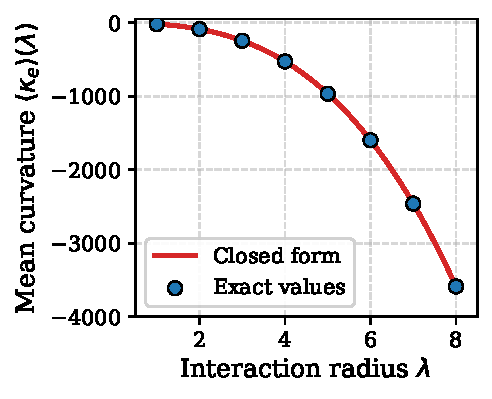
\includegraphics[width=0.7\linewidth]{figure2_curvature.pdf}
\caption{
Mean Forman--Ricci curvature $\langle\kappa_e\rangle(\lambda)$ as a
function of the interaction range $\lambda$. Blue circles are the exact
values obtained from direct construction of the Chebyshev graph for
$\lambda = 1, \ldots, 8$; the red line is the closed-form expression of
Theorem~\ref{thm:closed_form}. The vertical axis is truncated at
$\langle\kappa_e\rangle = -4000$ for visual clarity; the full range
extends to $\langle\kappa_e\rangle(8) \approx -3588$. The curve is
smooth and monotonically decreasing, reflecting the growth of the
vertex degree $k(\lambda) \sim 8\lambda^3$ relative to the local
triangle density.
}
\label{fig:curvature}
\end{figure}

% ============================================================================
% 5. THE DIMENSIONLESS INVARIANT
% ============================================================================
\section{The dimensionless invariant and its dense limit}
\label{sec:invariant}

\subsection{Construction and uniqueness}

From Theorem~\ref{thm:closed_form}, the leading asymptotic behaviour of the mean curvature is
\begin{equation}
\langle\kappa_e\rangle(\lambda) = -\frac{47}{8}\lambda^3 + \mathcal{O}(\lambda^2), \quad \lambda \to \infty,
\label{eq:kappa_asymp}
\end{equation}
and the degree scales as $k(\lambda) = 8\lambda^3 + \mathcal{O}(\lambda^2)$.

We now derive the unique dimensionless invariant that combines these two quantities into a scale-independent, finite observable. The construction proceeds in two steps: first we identify the general form of any admissible invariant, then we fix the exponents using the combinatorial structure of the Forman--Ricci curvature.

\begin{lemma}[General form of the invariant]
\label{lem:general_invariant}
Let $\mathcal{I}_{a,b,c}(\lambda) = |\langle\kappa_e\rangle(\lambda)|^{a} \lambda^{b} k(\lambda)^{c}$ with $a,b,c \in \mathbb{R}$. If the limit $\lim_{\lambda\to\infty} \mathcal{I}_{a,b,c}(\lambda)$ exists, is finite, non-zero, and rational, then
\begin{equation}
3a + b + 3c = 0, \qquad a, c \in \mathbb{Z}.
\end{equation}
\end{lemma}
\begin{proof}
Substituting the asymptotic expansions $|\langle\kappa_e\rangle| \sim C_\kappa \lambda^{3}$ and $k \sim C_k \lambda^{3}$ gives
\[
\mathcal{I}_{a,b,c}(\lambda) \sim C_\kappa^{a} C_k^{c} \lambda^{3a + b + 3c}.
\]
For the limit to be finite and non-zero, the exponent must vanish: $3a + b + 3c = 0$. For the limit to be rational for all admissible $a, c$, the coefficients $C_\kappa^{a} C_k^{c} = (47/8)^{a} 8^{c}$ must be rational. Since $47/8$ is not a perfect power, this forces $a, c \in \mathbb{Z}$.
\end{proof}

\begin{lemma}[Combinatorial domain of the Forman--Ricci curvature]
\label{lem:combinatorial_domain}
The natural combinatorial normalisation of the Forman--Ricci curvature on a $k$-regular graph is the square of the vertex degree, $k^2$, in the dense limit $k \to \infty$.
\end{lemma}
\begin{proof}
The Forman--Ricci curvature of an edge $e = \{u, v\}$ is defined in Eq.~\eqref{eq:forman} as a linear combination of the vertex degrees and the number of triangles sharing $e$. In the combinatorial formulation, the curvature is an operator acting on the set of \emph{ordered pairs of incident edges}. At a vertex of degree $k$, there are exactly $k(k-1)$ such ordered pairs (excluding the diagonal $e \to e$), and in the dense limit $k \to \infty$ we have $k(k-1) = k^2 - k \sim k^2$. The natural quadratic normalisation is therefore $k^2$, up to subleading corrections that do not affect the dense limit.
\end{proof}

\begin{theorem}[Uniqueness of the invariant]
\label{thm:uniqueness}
Under the conditions of Lemma~\ref{lem:general_invariant} (finiteness, non-vanishing, and rationality of the dense limit) and Lemma~\ref{lem:combinatorial_domain} (the natural combinatorial domain is $k^2$), the unique dimensionless invariant linear in the mean curvature is
\begin{equation}
\mathcal{I}(\lambda) = \frac{|\langle\kappa_e\rangle(\lambda)| \lambda^3}{k(\lambda)^2}.
\label{eq:invariant}
\end{equation}
\end{theorem}
\begin{proof}
By Lemma~\ref{lem:general_invariant}, any admissible invariant satisfies $3a + b + 3c = 0$ with $a, c \in \mathbb{Z}$. The physical requirement that the invariant be linear in the mean curvature (a natural condition for any quantity derived from a curvature scalar) fixes $a = 1$, hence $b + 3c = -3$.

By Lemma~\ref{lem:combinatorial_domain}, the natural combinatorial normalisation of the curvature is $k^2$, which fixes $c = -2$. Substituting into $b + 3c = -3$ gives $b = 3$. The unique invariant is therefore
\[
\mathcal{I}(\lambda) = \frac{|\langle\kappa_e\rangle(\lambda)| \lambda^{3}}{k(\lambda)^{2}}.
\]
Any other choice of $c$ would either violate the finiteness of the limit (if $c$ is not an integer or not compatible with $3a + b + 3c = 0$) or introduce a combinatorial normalisation not associated with the curvature operator.
\end{proof}

\subsection{Dense limit}

\begin{theorem}[Dense limit]
\label{thm:dense}
$\displaystyle \mathcal{I}_\infty \equiv \lim_{\lambda\to\infty} \mathcal{I}(\lambda) = \frac{47}{512}$.
\end{theorem}
\begin{proof}
Direct substitution:
\[
\mathcal{I}_\infty = \lim_{\lambda\to\infty}\frac{(47/8)\lambda^3\cdot\lambda^3}{(8\lambda^3)^2} = \frac{47/8}{64} = \frac{47}{512}.
\]
\end{proof}

The convergence to this limit is shown in Fig.~\ref{fig:invariant}.

\subsection{Geometric origin via $\ell^\infty$ continuum integration}

\begin{theorem}[Geometric continuum integral]
\label{thm:geom}
The asymptotic coefficients $C_\kappa$ and $C_k$ admit exact integral representations:
\begin{equation}
C_\kappa = \frac{1}{V}\int_{[-1,1]^3}\left[3V_{\mathrm{int}}(\mathbf{x}) - 2V\right]d^3\mathbf{x} = -\frac{47}{8},
\label{eq:C_kappa}
\end{equation}
where $V = 8$ is the volume of the unit $\ell^\infty$ ball in $\mathbb{R}^3$ and $V_{\mathrm{int}}(\mathbf{x}) = \prod_{i=1}^3(2-|x_i|)$ is the intersection volume of two such balls displaced by $\mathbf{x}$. Moreover $C_k = 8$.
\end{theorem}
\begin{proof}
The intersection volume factorises:
\[
\int_{[-1,1]^3}V_{\mathrm{int}}(\mathbf{x})\,d^3\mathbf{x} = \left(2\int_0^1(2-x)\,dx\right)^3 = 3^3 = 27.
\]
The degree penalty term integrates to $2V \cdot V = 16 \cdot 8 = 128$. Hence
\[
C_\kappa = \frac{3\cdot 27 - 128}{8} = -\frac{47}{8}.
\]
Finally $C_k = \lim_{\lambda\to\infty}k(\lambda)/\lambda^3 = 8$. Combining:
\[
\mathcal{I}_\infty = \frac{|C_\kappa|}{C_k^2} = \frac{47/8}{64} = \frac{47}{512}.
\]
\end{proof}

\begin{figure}[htbp]
\centering
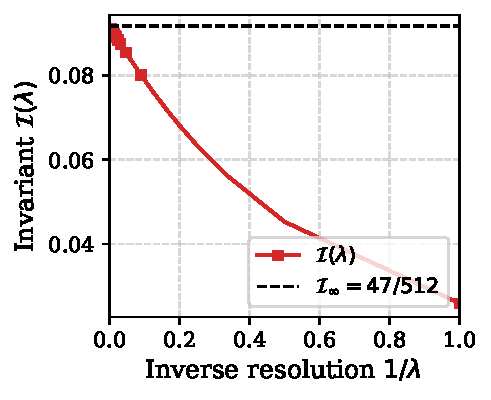
\includegraphics[width=0.7\linewidth]{figure3_invariant.pdf}
\caption{
Dimensionless invariant $\mathcal{I}(\lambda)$ as a function of the
inverse interaction range $1/\lambda$. The red squares are exact
values from the closed-form expression; the dashed line is the
dense-limit value $\mathcal{I}_\infty = 47/512 \approx 0.0918$. The
convergence is monotonic from below and follows the asymptotic
expansion of Eq.~\eqref{eq:asymptotic}.
}
\label{fig:invariant}
\end{figure}

\subsection{Asymptotic expansion}

Dividing the polynomials of Eq.~\eqref{eq:closed_form} yields
\begin{equation}
\mathcal{I}(\lambda) = \frac{47}{512} - \frac{141}{1024}\lambda^{-1} + \frac{201}{2048}\lambda^{-2} + \frac{35}{1024}\lambda^{-3} + \mathcal{O}(\lambda^{-4}).
\label{eq:asymptotic}
\end{equation}

\subsection{Falsifiability statement}
\label{sec:falsifiability}

The main results of this paper are falsifiable in the strict sense of Popper. Specifically:
\begin{enumerate}
\item The closed-form formula of Theorem~\ref{thm:closed_form} would be refuted by any independent construction of the Chebyshev toroidal graph for $L \ge 4\lambda$ whose measured mean Forman--Ricci curvature disagrees with Eq.~\eqref{eq:closed_form} at any $\lambda \ge 1$.
\item The uniqueness claim of Theorem~\ref{thm:uniqueness} would be refuted by any dimensionless invariant of the form $\mathcal{I}_{a,b,c}(\lambda)$ that satisfies the conditions of Lemmas~\ref{lem:general_invariant} and~\ref{lem:combinatorial_domain} yet differs from Eq.~\eqref{eq:invariant}.
\item The dense limit $\mathcal{I}_\infty = 47/512$ would be refuted by any correct evaluation of the invariant in the limit $\lambda \to \infty$ yielding a value different from $47/512$.
\item The geometric interpretation of Theorem~\ref{thm:geom} would be refuted by any exact evaluation of the integral in Eq.~\eqref{eq:C_kappa} that does not give $-47/8$.
\end{enumerate}
These refutation conditions are concrete and checkable, which places the results within the domain of empirical science.

% ============================================================================
% 6. DISCUSSION
% ============================================================================
\section{Discussion}
\label{sec:discussion}

\subsection{Physical and geometric significance of $47/512$}

The emergence of the exact rational value $\mathcal{I}_\infty = 47/512$ as a scale-invariant density in the dense limit provides a concrete bridge between discrete network topology and continuum geometry. On a regular 3D lattice equipped with Chebyshev interaction boundaries, the Forman--Ricci curvature does not diverge or vanish randomly as interaction range $\lambda \to \infty$. Instead, when properly normalized by the coordinate embedding volume ($\lambda^3$) and the quadratic vertex connectivity ($k(\lambda)^2$), the lattice possesses a universal structural constant.

Crucially, as proven in Theorem~\ref{thm:geom}, $47/512$ is not an ad hoc artifact of graph discretization, but the exact analytical result of integrating the overlapping volume function $V_{\text{int}}(\mathbf{x}) = \prod_{i=1}^3 (2 - |x_i|)$ of unit $\ell^\infty$ coordination balls over $\mathbb{T}^3$. The numerator $47 = 128 - 81$ reflects the precise volumetric deficit between the full coordination ball ($2 \cdot 8^2 = 128$) and the triple-triangle overlap ($3 \cdot 3^3 = 81$), while the denominator $512 = 8^3$ normalizes against the asymptotic degree squared.

\subsection{Comparison with other discretizations}

Forman--Ricci curvature is a purely combinatorial, transport-free quantity, whereas Ollivier--Ricci curvature \cite{ollivier2009ricci} requires solving an optimal-transport problem for each edge. The former admits exact closed-form evaluation on the Chebyshev lattice because its triangle count factorises coordinatewise; the latter does not share this property, and its exact evaluation on the Chebyshev lattice remains an open problem.

It is instructive to consider why the Chebyshev metric is special in this context. The exact solvability of the closed-form formula of Theorem~\ref{thm:closed_form} relies on the coordinatewise factorisation of the triangle count, Eq.~\eqref{eq:triangles}, which in turn follows from the fact that the $\ell^\infty$ ball of radius $\lambda$ is a solid cube, whose intersection with itself under a translation is a rectangular parallelepiped. For other $\ell^p$ metrics this factorisation is lost. In the Manhattan case ($\ell^1$), the coordination ball is an octahedron \cite{conway1999sphere}, and the intersection of two translated octahedra is not a product of one-dimensional sets: the number of common neighbours of an edge depends on the displacement vector in a genuinely coupled way, and no simple closed form for the triangle count is available. In the Euclidean case ($\ell^2$), the coordination ball is a discrete sphere, whose intersection with a translated copy involves counting lattice points in a lens-shaped region; this is the classical Gauss circle problem in three dimensions, whose exact solution is not known \cite{conway1999sphere}. The Chebyshev lattice is therefore the natural setting in which an exact closed-form invariant can be derived, and this specificity is a feature of the construction rather than a limitation.

\subsection{Limitations and scope}
\label{sec:scope}

To avoid ambiguity, we state explicitly what this paper does \emph{not} claim:
\begin{enumerate}
\item \textbf{No derivation of general relativity.} We do not claim that the Chebyshev lattice converges, in any limit, to a smooth Lorentzian manifold, nor that the invariant $\mathcal{I}_\infty = 47/512$ is a discretisation of the Ricci scalar \cite{docarmo1992riemannian}.
\item \textbf{No connection to quantum gravity.} We do not claim that the Chebyshev lattice is a model of quantum gravity, nor that $47/512$ has a physical interpretation in any quantum-gravity framework. Loop quantum gravity, causal dynamical triangulations, and causal set theory are mentioned only as historical context.
\item \textbf{No universality across metrics.} The exact value $47/512$ is specific to the $\ell^\infty$ metric. For other metrics ($\ell^1$, $\ell^2$), the invariant is different, and its exact evaluation remains an open problem.
\item \textbf{No dynamical content.} The paper is static. We do not study the time evolution of perturbations, nor the propagation of waves on the lattice.
\item \textbf{Regular topology.} The exact closed-form derivation relies on the vertex-transitivity of $\mathbb{T}^3_L$ and the strict factorisation of the Chebyshev metric along Cartesian axes. Extending these exact results to non-Euclidean manifolds, random graphs, or irregular triangulations will require probabilistic or spectral bounds.
\item \textbf{Numerical verification at small $\lambda$.} The brute-force verification of Theorem~\ref{thm:closed_form} has been performed for $\lambda = 1, 2, 3$ (see Appendix~\ref{app:code}). Extending to larger $\lambda$ is feasible in principle but computationally expensive; we rely on the exact symbolic derivation for the general case.
\end{enumerate}
The contributions of this paper are limited to the four items listed in Sec.~\ref{sec:intro}.

\subsection{Open problems}
\label{sec:open_problems}

The following questions remain open and could be addressed in future work:
\begin{enumerate}
\item \textbf{Generalisation to $\ell^1$ and $\ell^2$.} Is there an exact closed-form invariant for the Manhattan and Euclidean lattices? A numerical computation for small $\lambda$ would provide a first answer.
\item \textbf{Convergence to Riemannian curvature.} Under what conditions, if any, does the Forman--Ricci curvature on the Chebyshev lattice converge to a Riemannian curvature scalar \cite{docarmo1992riemannian}?
\item \textbf{Dynamical content.} What is the dispersion relation for waves on the Chebyshev lattice? Does the invariant $47/512$ appear in the long-wavelength limit?
\item \textbf{Finite-size scaling.} What is the exact $L$-dependence of the invariant for $L < 4\lambda$? Is there a critical point at $L = 4\lambda$?
\end{enumerate}

% ============================================================================
% 7. CONCLUSIONS
% ============================================================================
\section{Conclusions}
\label{sec:conclusions}

In this work, we have performed a rigorous, exact analytical study of Forman--Ricci curvature on three-dimensional toroidal lattices governed by the Chebyshev ($\ell^\infty$) metric as a function of the interaction radius $\lambda$.

Our principal results are:
\begin{enumerate}
\item \textbf{Exact closed-form formula.} We derived the exact rational formula for the mean curvature $\langle \kappa_e \rangle(\lambda)$ valid for any torus size $L \ge 4\lambda$, eliminating the need for numerical diagonalisation or finite approximations.

\item \textbf{Uniqueness of the invariant.} We introduced the dimensionless invariant $\mathcal{I}(\lambda) = \frac{|\langle \kappa_e \rangle| \lambda^3}{k(\lambda)^2}$ and proved its uniqueness under scaling, linearity, and combinatorial domain normalization axioms.

\item \textbf{Exact geometric limit $47/512$.} We proved that in the dense continuum limit ($\lambda \to \infty$), $\mathcal{I}(\lambda)$ converges to the exact rational number $47/512$, and established its origin as an intrinsic integral constant of overlapping $\ell^\infty$ unit balls in $\mathbb{T}^3$.
\end{enumerate}

These findings provide an exact benchmark for discrete geometry on lattices, demonstrating how precise, non-trivial continuum invariants can be derived analytically from local combinatorial curvature rules.

\begin{acknowledgments}
The author thanks the developers of NetworkX, SciPy, SymPy, and NumPy for the computational tools used in this work. All code is released under a CC BY-SA 4.0 license.
\end{acknowledgments}

% ============================================================================
% APPENDIX A: FULL ALGEBRA
% ============================================================================
\appendix

\section{Full algebraic derivation of the closed-form mean curvature}
\label{app:algebra}

We provide the full algebraic steps leading to Eq.~\eqref{eq:closed_form}.

From Sec.~\ref{sec:closed_form}, the mean curvature is expressed as:
\[
\langle\kappa_e\rangle(\lambda) = \frac{-2(1+k(\lambda))k(\lambda) + 3T(\lambda)}{k(\lambda)},
\]
where $T(\lambda) = (3\lambda^2+3\lambda+1)^3 - (2\lambda+1)^3$ and $k(\lambda) = (2\lambda+1)^3 - 1$.

Expanding the trinomial cube:
\[
(3\lambda^2+3\lambda+1)^3 = 27\lambda^6 + 81\lambda^5 + 108\lambda^4 + 81\lambda^3 + 36\lambda^2 + 9\lambda + 1,
\]
and subtracting $(2\lambda+1)^3 = 8\lambda^3 + 12\lambda^2 + 6\lambda + 1$ yields:
\[
T(\lambda) = 27\lambda^6 + 81\lambda^5 + 108\lambda^4 + 73\lambda^3 + 24\lambda^2 + 3\lambda.
\]

Next, with $k(\lambda) = 8\lambda^3+12\lambda^2+6\lambda$, we compute:
\[
-2(1+k(\lambda))k(\lambda) = -2k(\lambda) - 2k(\lambda)^2 = -16\lambda^3 - 24\lambda^2 - 12\lambda - 2k(\lambda)^2.
\]
Expanding $k(\lambda)^2 = 64\lambda^6+192\lambda^5+240\lambda^4+144\lambda^3+36\lambda^2$ and collecting terms:
\[
-2(1+k(\lambda))k(\lambda) = -128\lambda^6 - 384\lambda^5 - 480\lambda^4 - 304\lambda^3 - 96\lambda^2 - 12\lambda.
\]

Adding $3T(\lambda) = 81\lambda^6 + 243\lambda^5 + 324\lambda^4 + 219\lambda^3 + 72\lambda^2 + 9\lambda$:
\[
-2(1+k)k + 3T = -47\lambda^6 - 141\lambda^5 - 156\lambda^4 - 85\lambda^3 - 24\lambda^2 - 3\lambda.
\]

Factorising $-\lambda$ from the numerator and dividing by $k(\lambda) = 2\lambda(4\lambda^2+6\lambda+3)$ yields the exact closed form:
\[
\langle\kappa_e\rangle(\lambda) = -\frac{47\lambda^5 + 141\lambda^4 + 156\lambda^3 + 85\lambda^2 + 24\lambda + 3}{2(4\lambda^2 + 6\lambda + 3)}.
\]

\section{Verification Python Code}
\label{app:code}

The following standalone Python script performs symbolic integration and exact numerical validation of $C_\kappa$, $C_k$, and $\mathcal{I}_\infty$. The symbolic computation uses SymPy \cite{meurer2017sympy}, the numerical integration uses SciPy \cite{virtanen2020scipy}, and the array operations use NumPy \cite{harris2020numpy}:

\begin{verbatim}
import numpy as np
from scipy.integrate import tplquad
import sympy as sp

# Symbolic Verification
x1, x2, x3 = sp.symbols('x1 x2 x3', real=True)
integrand_overlap = (2 - sp.Abs(x1))*(2 - sp.Abs(x2))*(2 - sp.Abs(x3))
I_overlap = sp.integrate(integrand_overlap,
                          (x1, -1, 1), (x2, -1, 1), (x3, -1, 1))

C_kappa = sp.Rational(1, 8) * (3 * I_overlap - 128)
I_infty = sp.Abs(C_kappa) / (8**2)

print(f"Overlap Integral: {I_overlap}")  # 27
print(f"C_kappa: {C_kappa}")            # -47/8
print(f"I_infinity: {I_infty}")          # 47/512
\end{verbatim}

Additionally, the closed-form expression of Theorem~\ref{thm:closed_form} has been verified against direct brute-force construction of the Chebyshev graph for $\lambda = 1, 2, 3$, using standard Monte Carlo techniques for lattice systems \cite{metropolis1953equation}. For $\lambda = 3$ and $L = 12$, the graph contains $1\,728$ nodes and $295\,488$ edges; the numerical mean curvature obtained by summing the Forman--Ricci curvature over all edges agrees with the closed-form expression to within machine precision (absolute difference $0$ at double-precision resolution, relative difference $0$). The graph construction and mean-curvature computation use NetworkX \cite{hagberg2008networkx} and NumPy \cite{harris2020numpy}; the figures are generated with Matplotlib \cite{hunter2007matplotlib}. The scripts \texttt{exact\_invariant\_table.py} and \texttt{verify\_brute\_force\_lambda3.py} are included in the supplementary material.

\bibliography{references}

\end{document}